\section*{Reactor design}
Transitioning from batch to continuous process requires a complete redesign of the reactors that are commonly used in the industry today. Nitration of toluene produces 3 isomers of nitrotoluene, but only ONT and PNT were of commercial interest. The reactor must be capable of handling 816 tonnes of ONT and 841 tonnes of PNT throughput per annum. To meet this annual demand while minimising safety risk and maximising performance of the reactor, Nitroma developed a novel approach of using a Heat Exchanger Reactor (HEX Reactor) for the nitration of toluene.

%general overview
A key aspect of innovation in the nitration reactor is its ability to have a robust temperature control within its compact design. This was achieved by having a triple concentric tube arrangement. Each of the 7 reaction tubes were surrounded by an outer primary cooling water jacket, with an additional secondary concentric pipe through the centre of each reaction tube. 

Silicon 

%kinetics
The kinetics of the zeolite-catalysed nitration reaction were determined using literature data and the Arrhenius equation. To allow for more accurate modelling, the rate equation for the production of each nitrotoluene isomer were determined. 
%modelling approach [andreas]
The model was implemented and optimised on COMSOL 5.6. 
-steps taken to model ( Brinkman) 

%optimisation [zong]
To ensure the reactor operates in optimal conditions, the following parameters were optimised: Concentric inner cooling pipe diameter and flowrate, direction of cooling water flow, \ch{HNO3} : Toluene inlet ratio and the total number of reaction tubes. The optimised values were used the final reactor design.

A further sensitivity analysis was performed on the cooling water inlet temperature since the temperature inside the reactor needs to be well-controlled at all times. Cooling water temperature was simulated to vary by \mypm $\Delta$ 5 K and the total length of reactor required to achieve 98\% conversion while keeping temperature below the safe limit of 363K was investigated. The cooling water is not expected to fluctuate to this degree since it is reused and mixed together from multiple cooling water streams in the plant, but taking a conservative approach increases the overall safety of Nitroma's plant in the worst case scenario. The optimal length was determined to be 4.2m. 


%mech design [loon]
The final reactor design can be seen in Figure \ref{fig:executivesummaryreactor}
\begin{figure}[h]
    \centering
    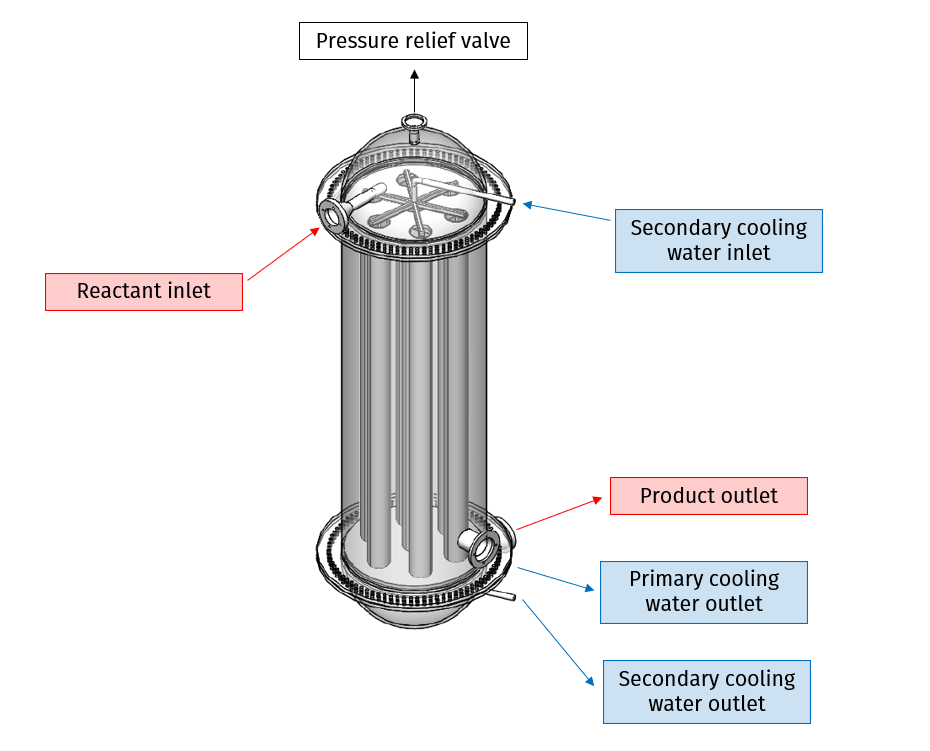
\includegraphics[width=0.7\linewidth]{chapters/0-executive-summary/figures/FYD executive sum.PNG}
    \caption{Mechanical design of nitration reactor}
    \label{fig:executivesummaryreactor}
\end{figure}